
This section examines how retrieval heads influence downstream tasks. 
Across the experiments we use Mistrial-7B-Instruct-v0.2~\citep{mistralv02} as it is a popular and strong open language model with 32K context length. 
We first show that retrieval heads explains the factuality of Needle-in-a-Haystack test. 
When the model can retrieve the needle, retrieval heads are always activated. 
When the model cannot retrieve the needle and hallucinate instead, retrieval heads are either partially activated or not activated. 
Then we show that retrieval heads significantly influence question answering that requires extracting the information from the input, but does not strongly influence tasks where the model directly produce answers based on its internal knowledge.
We further explore how retrieval heads influence more sophisticated reasoning behaviors like chain-of-thought~\citep{DBLP:conf/nips/Wei0SBIXCLZ22}.



\subsection{Retrieval Heads Explains Factuality in Needle-in-a-Haystack}
We start with a closer look at Needle-in-a-Haystack and  
construct an additional set of needle tests that are different from the three sets used for retrieval head detection. 
We gradually mask out the number of retrieval/ random heads and see how the model's behavior changes. 
As is shown in Fig.~\ref{fig:needle_mask}, masking out retrieval heads severely damages the model's Needle-in-a-Haystack performance, while masking out random heads shows much smaller performance impact. 
Notably, when increasing the number of masked heads K to 50 (about 5\% of the full number of heads), all models' needle test performance drop to below 50, showing that the top retrieval heads are responsible for most of the needle retrieval behavior. 


\begin{figure}[!t]
    \begin{minipage}[t]{0.3\textwidth}
        \vspace{0pt}
        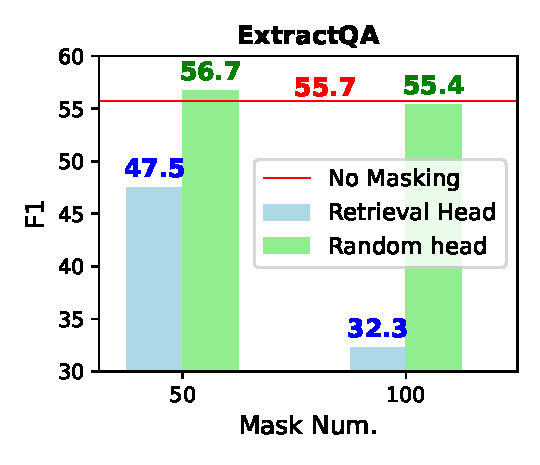
\includegraphics[width=\textwidth]{figures/task_qa.pdf}
        \caption{Masking out retrieval heads severely damages ExtractQA performance. 
        }
        \label{fig:task_qa}
    \end{minipage}
    \hfill
    \begin{minipage}[t]{0.66\textwidth}
        \vspace{0pt}
        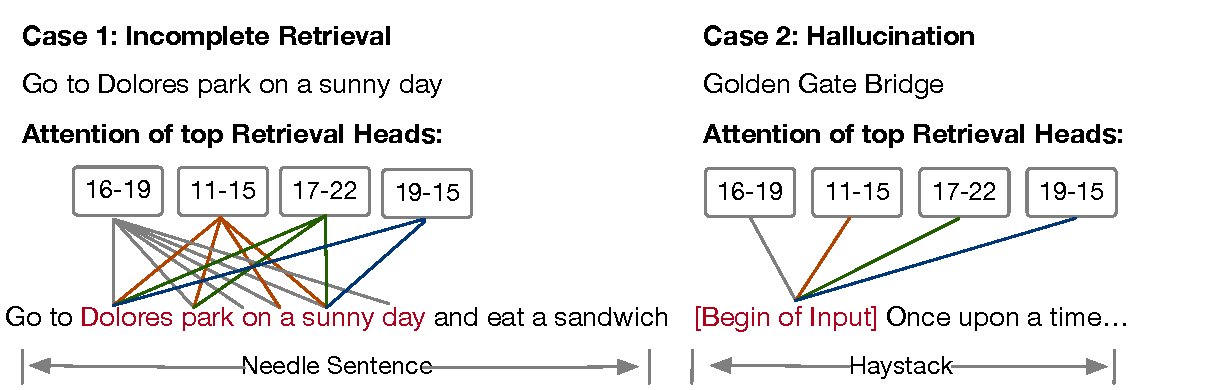
\includegraphics[width=\textwidth]{figures/wrong_head_case.pdf}
        \caption{When the model fails to retrieve the full needle, there are two typical errors:
(1) incomplete retrieval, where the retrieval heads miss part of the information ``eat a sandwich'';
(2) hallucination, where the retrieval heads attend to the initial tokens.
        }
        \label{fig:wrong_head_case}
    \end{minipage}
\end{figure}
We observe three types of error: (1) Incomplete retrieval, where models only captured partial information of the target and omitted key details; (2) Hallucination, where models generated hallucinated sentences; and (3) Wrong extraction, where models incorrectly retrieved irrelevant content from the haystack.
Without any masking, instances of wrong extraction occurred when retrieval heads were active but focused on incorrect sections. During hallucinated generation, retrieval heads predominantly attended to the initial token of the input, which is often known as "attention sink"~\citep{xiao2023efficient}, presumably dummy tokens that provide less meaningful signal.


As we increase the number of masked heads, initially, 
a small subset of the most robust retrieval heads are masked, and incomplete retrieval began to appear. 
In the absence of the strongest retrieval heads, the remaining weaker heads only managed to retrieve a fraction of the target information.
Metaphorically, each retrieval head holds a small piece of the "needle," yet these pieces cannot form a complete one, resulting in an incomplete final output. 
This phenomenon typically begins when the mask out heads of  retrieval score larger than 0.4.
As we further increase the number of mask, 
% In the second stage, as more retrieval heads are masked, 
hallucinations become more prevalent, signaling a complete failure of the retrieval capability.

\subsection{Influence on Extractive QA}
Now we study how retrieval heads influence more realistic tasks beyond Needle-in-a-Haystack. 
We use extractive QA as a test bed, as common usecase of long-context model where the user typically upload a pdf (research papers, finantial reports, legal documents, .etc) and ask questions about specific information within the document. 
To make sure the knowledge being asked does not exist in the model's internal knowledge, we synthesize an extractive QA dataset by selecting a set of \textit{up-to-date} news articles, extract a paragraph from it, and asking GPT-4 to produce a question-answer pair based on the extracted paragraph, similar to the evaluation conducted in~\citet{claude}. 
As illustrated in Figure~\ref{fig:task_qa},
randomly masking out non-retrieval heads demonstrated no significant impact on performance. 
Masking out retrieval heads led to a substantial decrease in F1 scores, with reductions of 9.2\% and 23.1\%.
These observations demonstrate that real-world document QA tasks heavily rely on the functionality of retrieval heads. 


\subsection{Chain-of-Thought Reasoning also Requires Retrieval Heads}
\begin{figure*}[t!]
\small
  \centering
  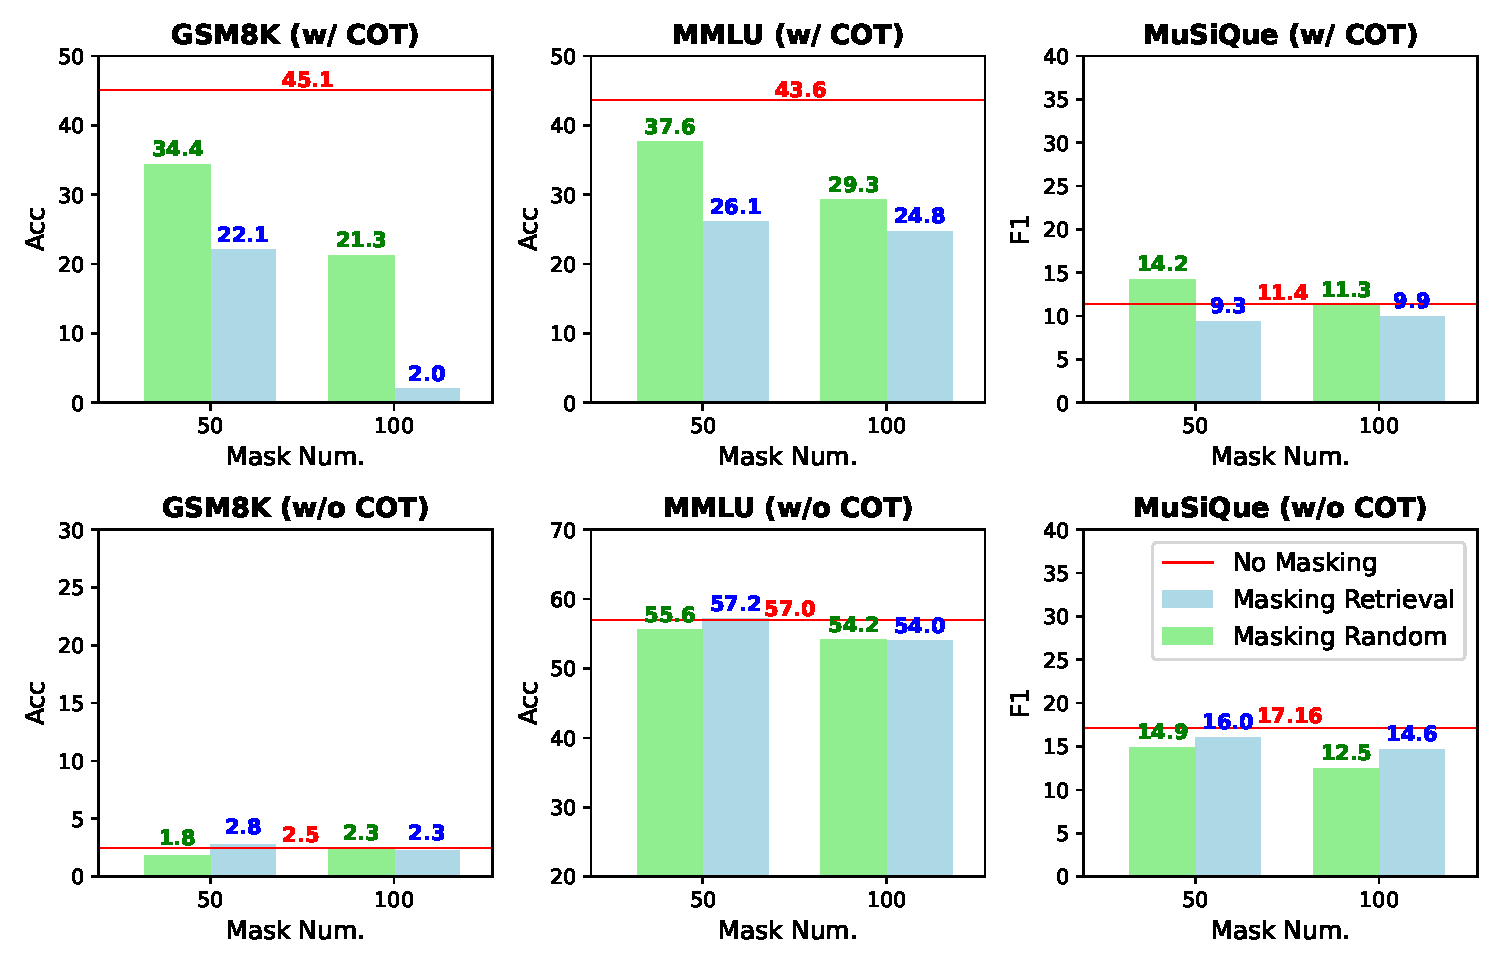
\includegraphics[width=1.0\linewidth]{figures/task_cot.pdf}
  \caption{Retrieval heads significantly influence tasks that require chain-of-thought reasoning. 
  This is because typically in a reasoning chain, the next step reasoning requires the model to refer to previous information. See Fig.~\ref{fig:gsm8k_error_case} for examples.
  }
  \label{fig:task_cot}
\end{figure*}

\begin{figure}[t!]
\small
  \centering
  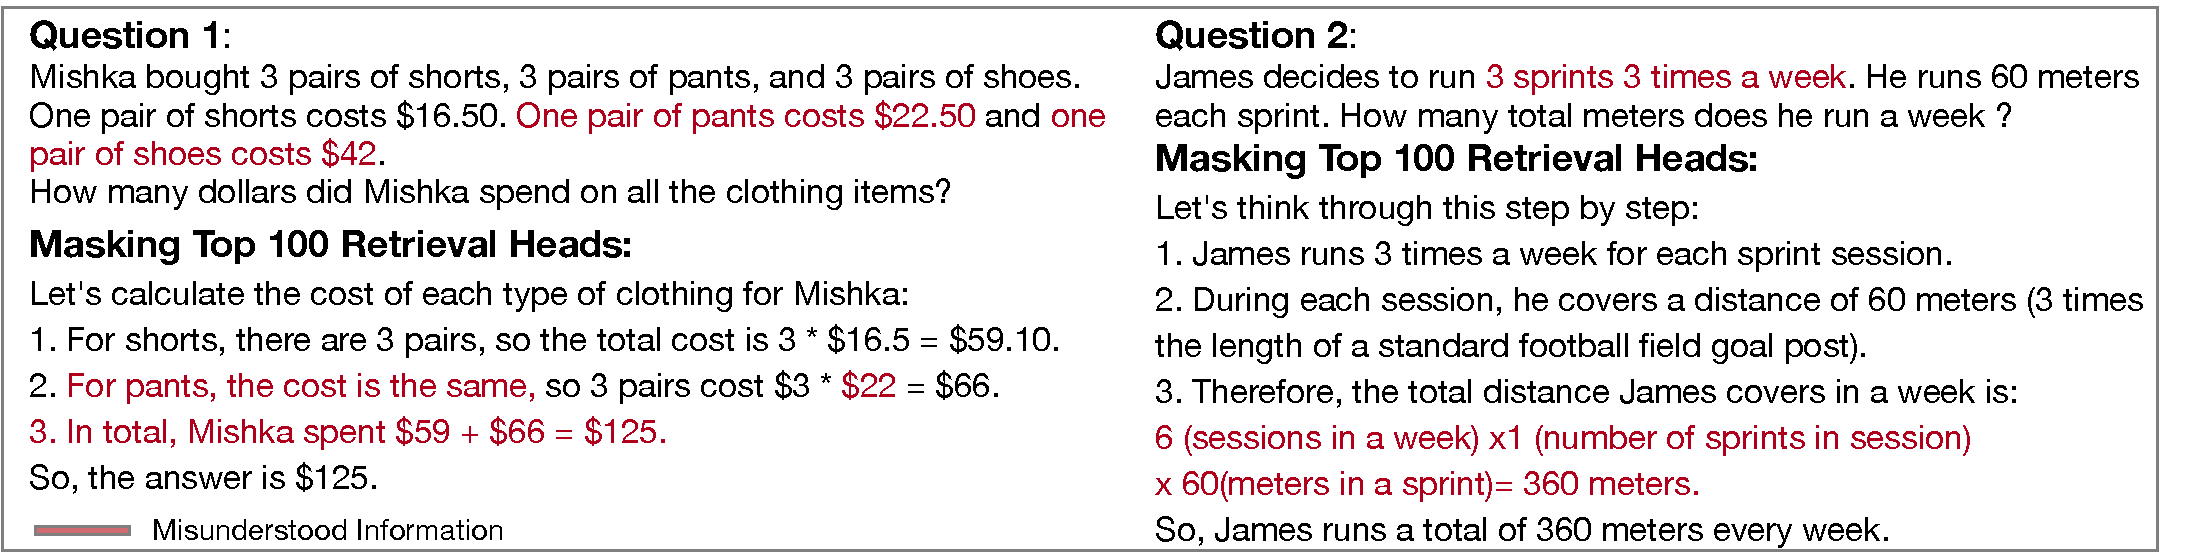
\includegraphics[width=\linewidth]{figures/case_cot.pdf}
  \caption{ 
  % Two cases of the generated CoT inferenced without retrieval heads from GSM8K.
  % Red lines are the  information  the language model failed to use, and its corresponded generation.  Blue lines are irrelevant  hallucinations
  % When masking out retrieval heads, 
  When we mask out retrieval heads, the model becomes ``blind'' to important information in the question description
  % the model fails to utilize important input information and hallucinates instead,
  resulting in incorrect reasoning chains. 
  }
  \label{fig:gsm8k_error_case}
\end{figure}
We test Mistrial-7B-Instruct-v0.2's performance on MMLU~\citep{hendrycks2020measuring}, MuSiQue and GSM8K~\citep{cobbe2021training}, with and without chain-of-thought reasoning. 
As is shown in Fig.~\ref{fig:task_cot}, 
if we use answer-only prompting (without CoT), masking out either retrieval or random heads do not really influence the performance, presumably because the model's generation is based on its internal knowledge primarily stored in the FFN layers~\citep{geva2020transformer}. 
For CoT styled reasoning, masking out retrieval heads signifantly influence the model's performance. 
Upon inspecting typically error cases (Fig.~\ref{fig:gsm8k_error_case}), we find out the model becomes ``blind'' to important input information and hallucinate instead. 
We find the relationship between CoT and retrieval heads particularly intriguing as it may offers deeper insights into model's complex reasoning performance. 
We leave more in-depth studies to future research.


